\subsection{Planar coil magnetic field}
The structure of a planar coil is very different from a standard one, as it is a flat structure with a spiral winding. The magnetic field generated by a planar coil is more complex than that of a standard coil, as the magnetic field is not concentrated in the center of the coil but is distributed over the entire surface of the coil. The magnetic field generated by a planar coil is represented in Figure \ref{fig: Spiral magn field}

\begin{figure}[th]
    \centering
    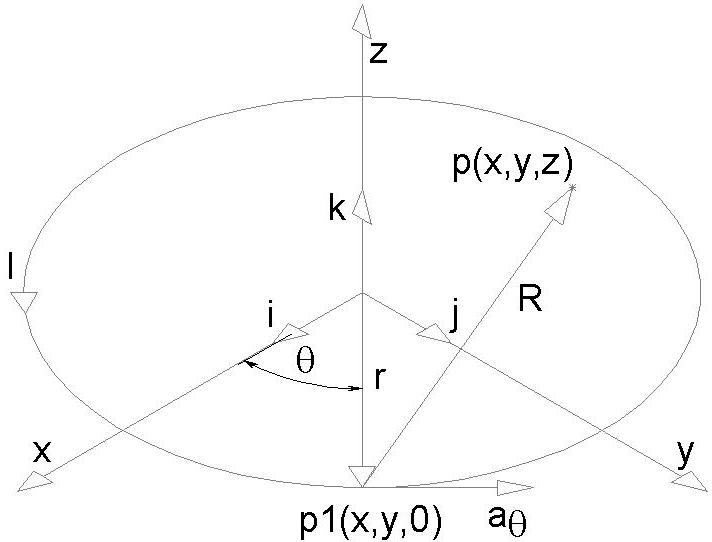
\includegraphics[scale=0.4]{Chapters/Chapter2/PCB_coils/Figures/coil_field_diagram.png} % TODO: Change image with svg
    \caption[Spiral magn field]{(c) Representation of the magnetic field generated by a circular spiral planar coil placed on an aluminum plate.\cite{Spiral_Coil_magn_field}}
    \label{fig: Spiral magn field}
\end{figure}

Then considering again the circular spiral structure, the magnetic field generated by a planar coil at its surface can be derived as

\begin{figure}
    \centering
    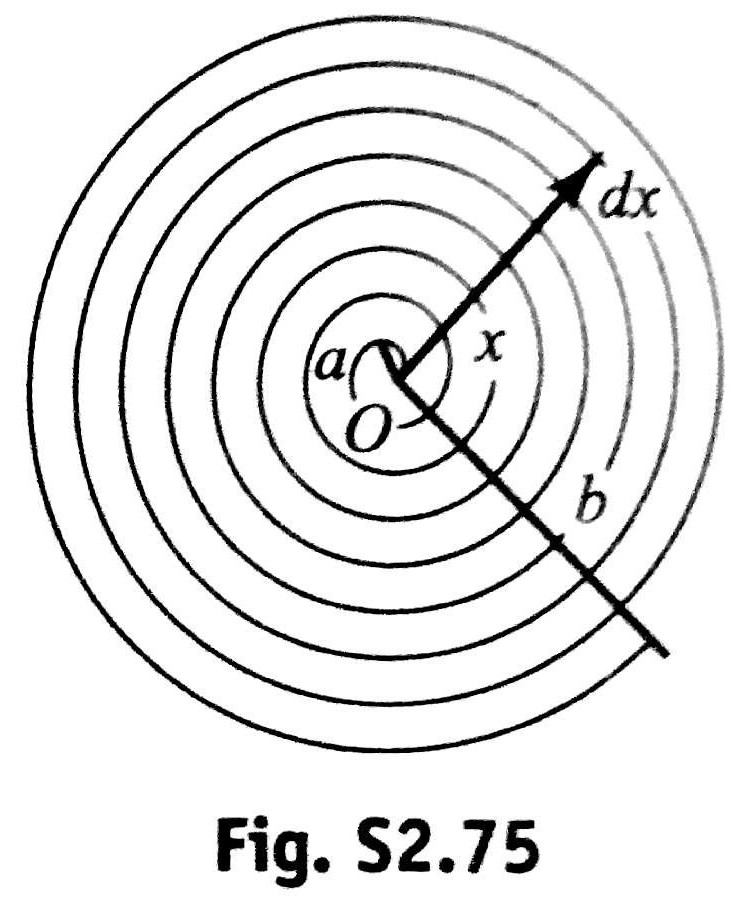
\includegraphics[scale=0.4]{Chapters/Chapter2/PCB_coils/Figures/spiral_windings.jpg} % TODO: Change picture with svg
    \caption[Coil spiral]{Circular spiral coil.}
    \label{fig: Coil spiral}
\end{figure}

\begin{equation}
    Bz = \frac{\mu N I}{2} \cdot \frac{\ln(\frac{b}{a})}{b-a} % https://www.youtube.com/watch?v=1bp9gGCSLc4 TODO: find a reference
    \label{eq: Spiral_magn_field}
\end{equation}

Where:
\begin{itemize}
    \item $Bz$ is the magnetic field on the z-axis [T]
    \item $\mu$ is the magnetic permeability of the medium [H/m]
    \item $n$ is the number of turns of the spiral
    \item $I$ is the current flowing through the wire [A]
    \item $b$ is the external radius of the spiral [m]
    \item $a$ is the internal radius of the spiral [m]
\end{itemize}

To then find the magnetic field at a distance $z$ from the center of the coil, we can use the equation \eqref{eq: Coil_magn_field} from the previous subsection and substitute the radius $r$ of the coil with   

\begin{equation}
    r' = \frac{b-a}{\ln\frac{b}{a}} \rightarrow B_z = \frac{\mu N I r'^2}{2(r'^2+z^2)^\frac{3}{2}} \label{eq: Spiral_magn_field_dist}
\end{equation}

